% vim: set ts=2 sw=2 noet:
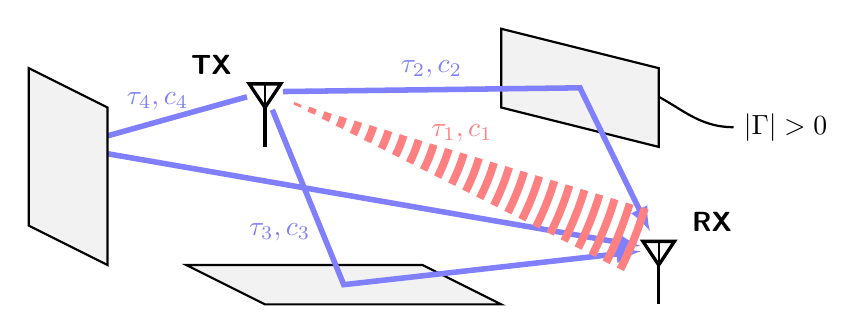
\begin{tikzpicture}[
			antenna/.pic = {
				\draw[very thick] (0,0) -- ++(2mm, 3mm) -- ++(-4mm,0) -- cycle;
				\draw[very thick] (0,0) -- ++(0,-5mm) coordinate (-mast) {};
				\draw[thick] (0,0) -- ++(0,3mm);
				\node[inner sep = 0pt, outer sep = 6pt] (-center) at (0,2mm) {};
			},
	]

	% Antennas
	\draw (0,2) pic (T) {antenna} node[above left = 3mm] {\sffamily\bfseries TX};
	\draw (5,0) pic (R) {antenna} node[above right = 3mm] {\sffamily\bfseries RX};

	% wall coefficients
	\draw[thick] (4.75, 2.25) to[out = -20, in = 180] ++(1.2,-.5) node[right] {\(|\Gamma| > 0\)};

	% walls
	\draw[thick, fill = lightgray!20] (3,2) -- ++(2,-.5) -- ++(0,1) -- ++(-2,.5) -- cycle;
	\draw[thick, fill = lightgray!20] (-1,0) -- ++(3,0) -- ++(1,-.5) -- ++(-3,0) -- cycle;


	% reflected signals
	\draw[line width = 2pt, blue!50!white, -latex] (T-center) -- node[above, pos = .5] {\(\tau_2,c_2\)} (4,2.25) -- (R-center);
	\draw[line width = 2pt, blue!50!white, -latex] (T-center) -- node[left, pos = .7] {\(\tau_3,c_3\)} (1,-.25) -- (R-center);
	\draw[line width = 2pt, blue!50!white, -latex] (T-center) -- node[above, pos = .5] {\(\tau_4,c_4\)} (-2.5,1.5) -- (R-center); 

	% another wall
	\draw[thick, fill = lightgray!20] (-2,0) -- ++(-1,.5) -- ++(0,2) --++(1,-.5) -- cycle;

	% LOS path
	\draw[line width = 1mm, red!50!white,
		decorate, decoration = {
			expanding waves, angle = 5, segment length = 2mm
		}
	] (T-center) -- node[above = 2mm, pos = .5] {\(\tau_1,c_1\)} (R-center);
\end{tikzpicture}
